\section{Results}
%example network
\FloatBarrier
\begin{figure}[htb!]
    \makebox[\textwidth][c]{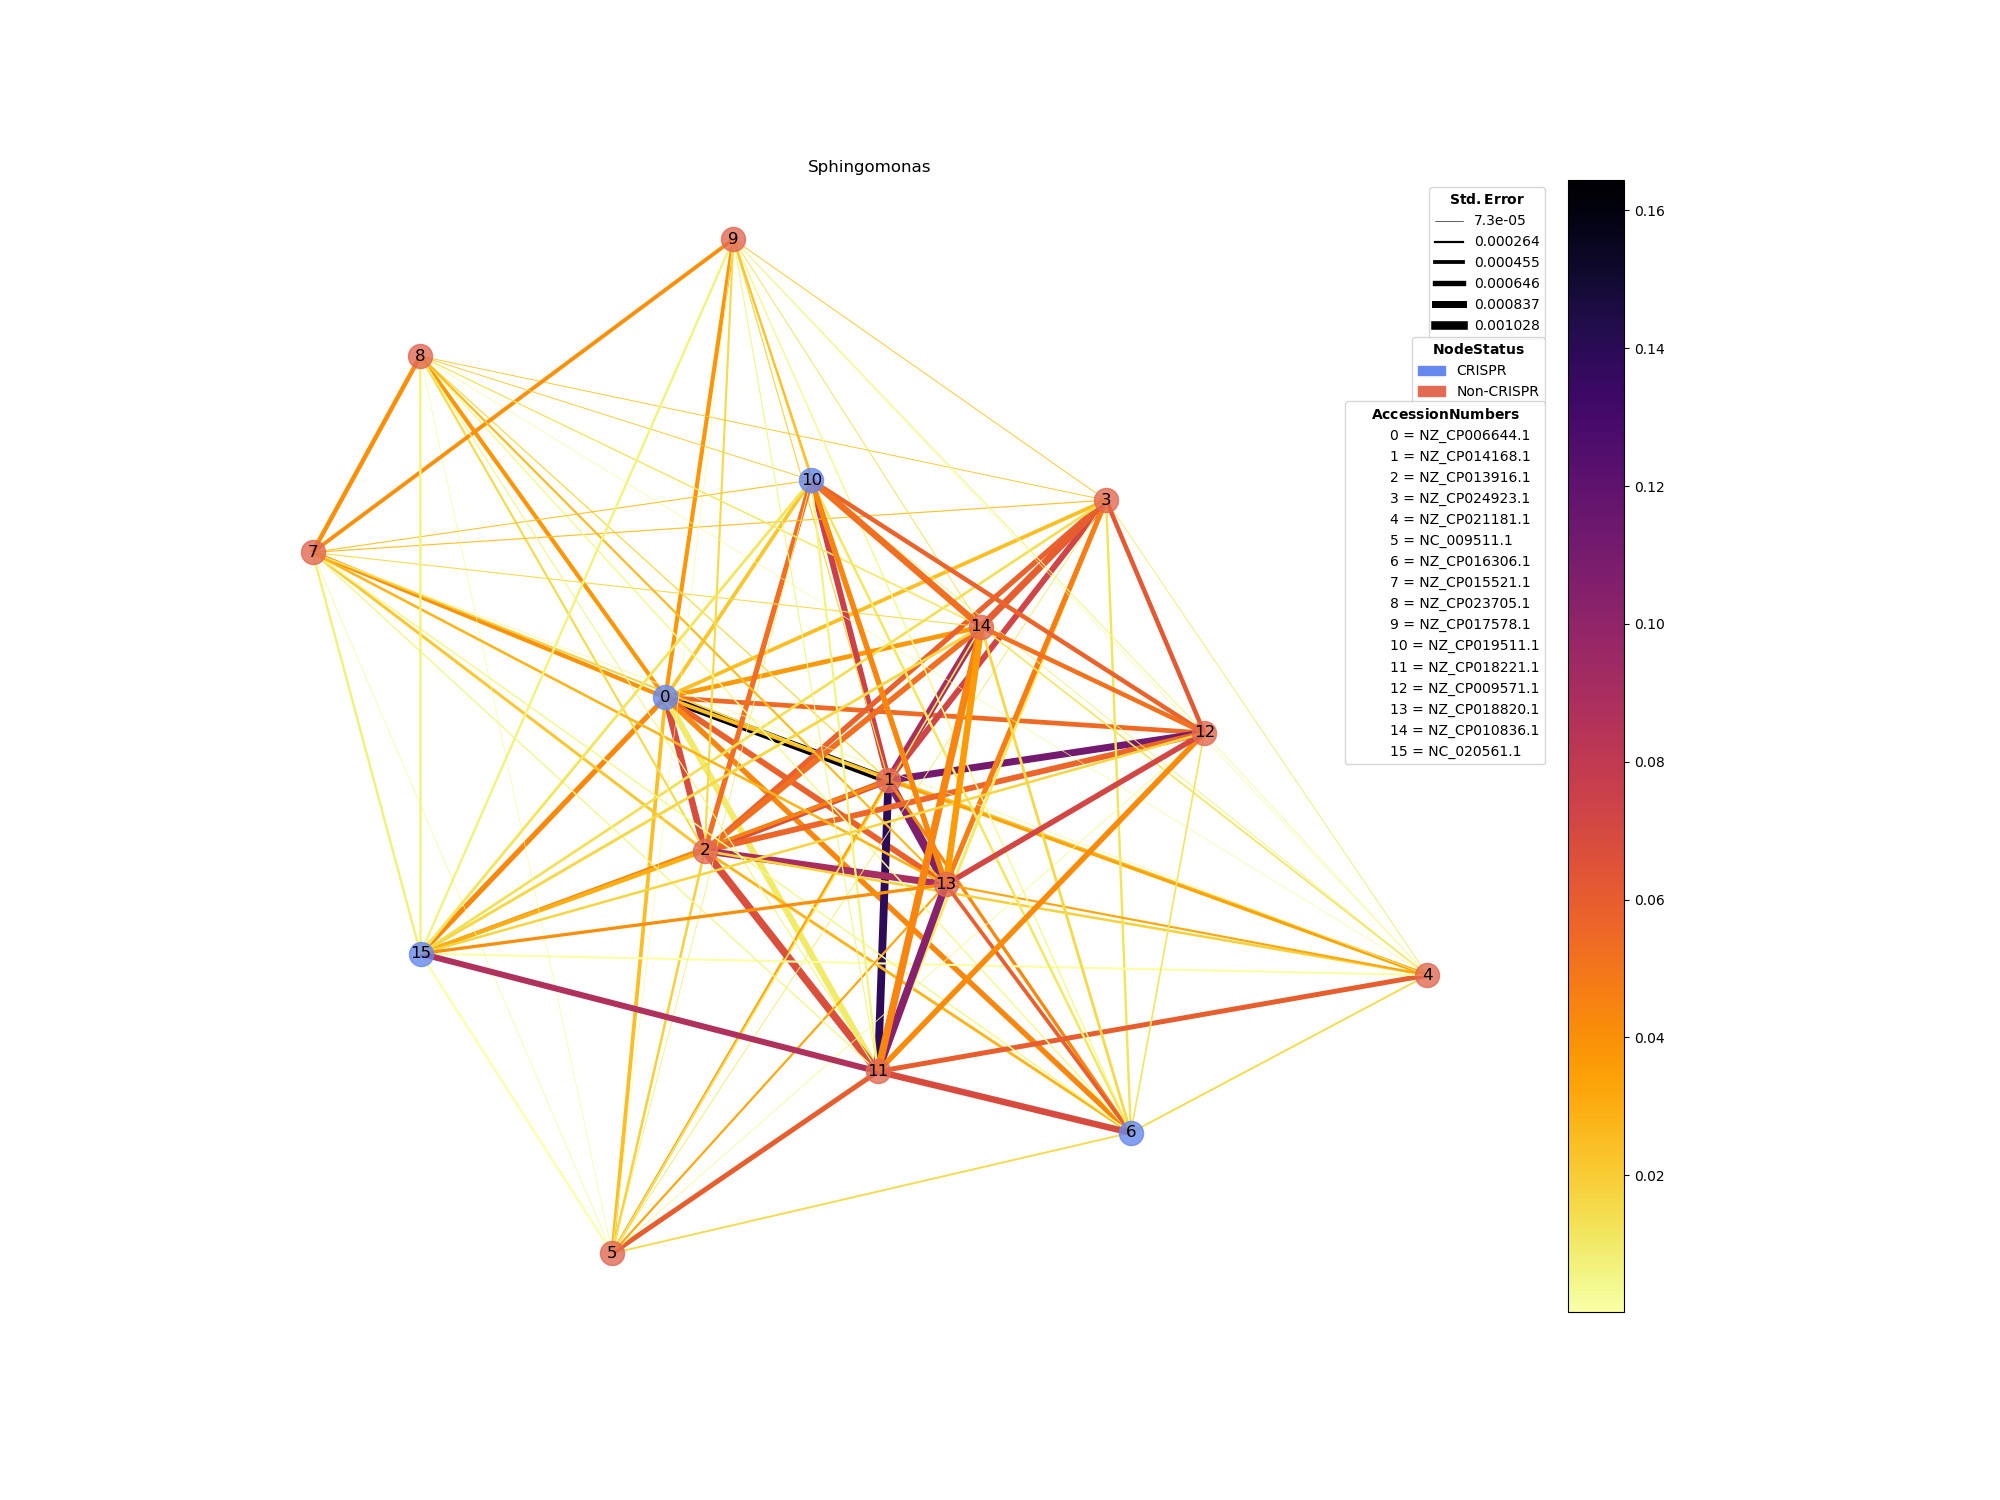
\includegraphics[width=1.3\linewidth]{network.png}}
    \caption{Example of a \ac{hgt} network produced by HiDe. This network is a ``consensus'' over 1000 bootstap replicate networks, produced from sampling gene trees. Each bootstrap replicate was produced from 50 randomly sampled gene trees froma a total of 376 individual gene trees. Blue nodes were cassified as having a \ac{crsp} system, red nodes were not. Color represents the fraction of genes examined that were transfered along that edge. Width represents the standard error of the edge value over the 1000 bootstraps. (Note the maximum value for an edge is 1.00, meaning all examined genes were transfered along that edge)}
    \label{net}
\end{figure}
\FloatBarrier
%degree bar
\FloatBarrier
\begin{figure}[htb!]
    \makebox[\textwidth][c]{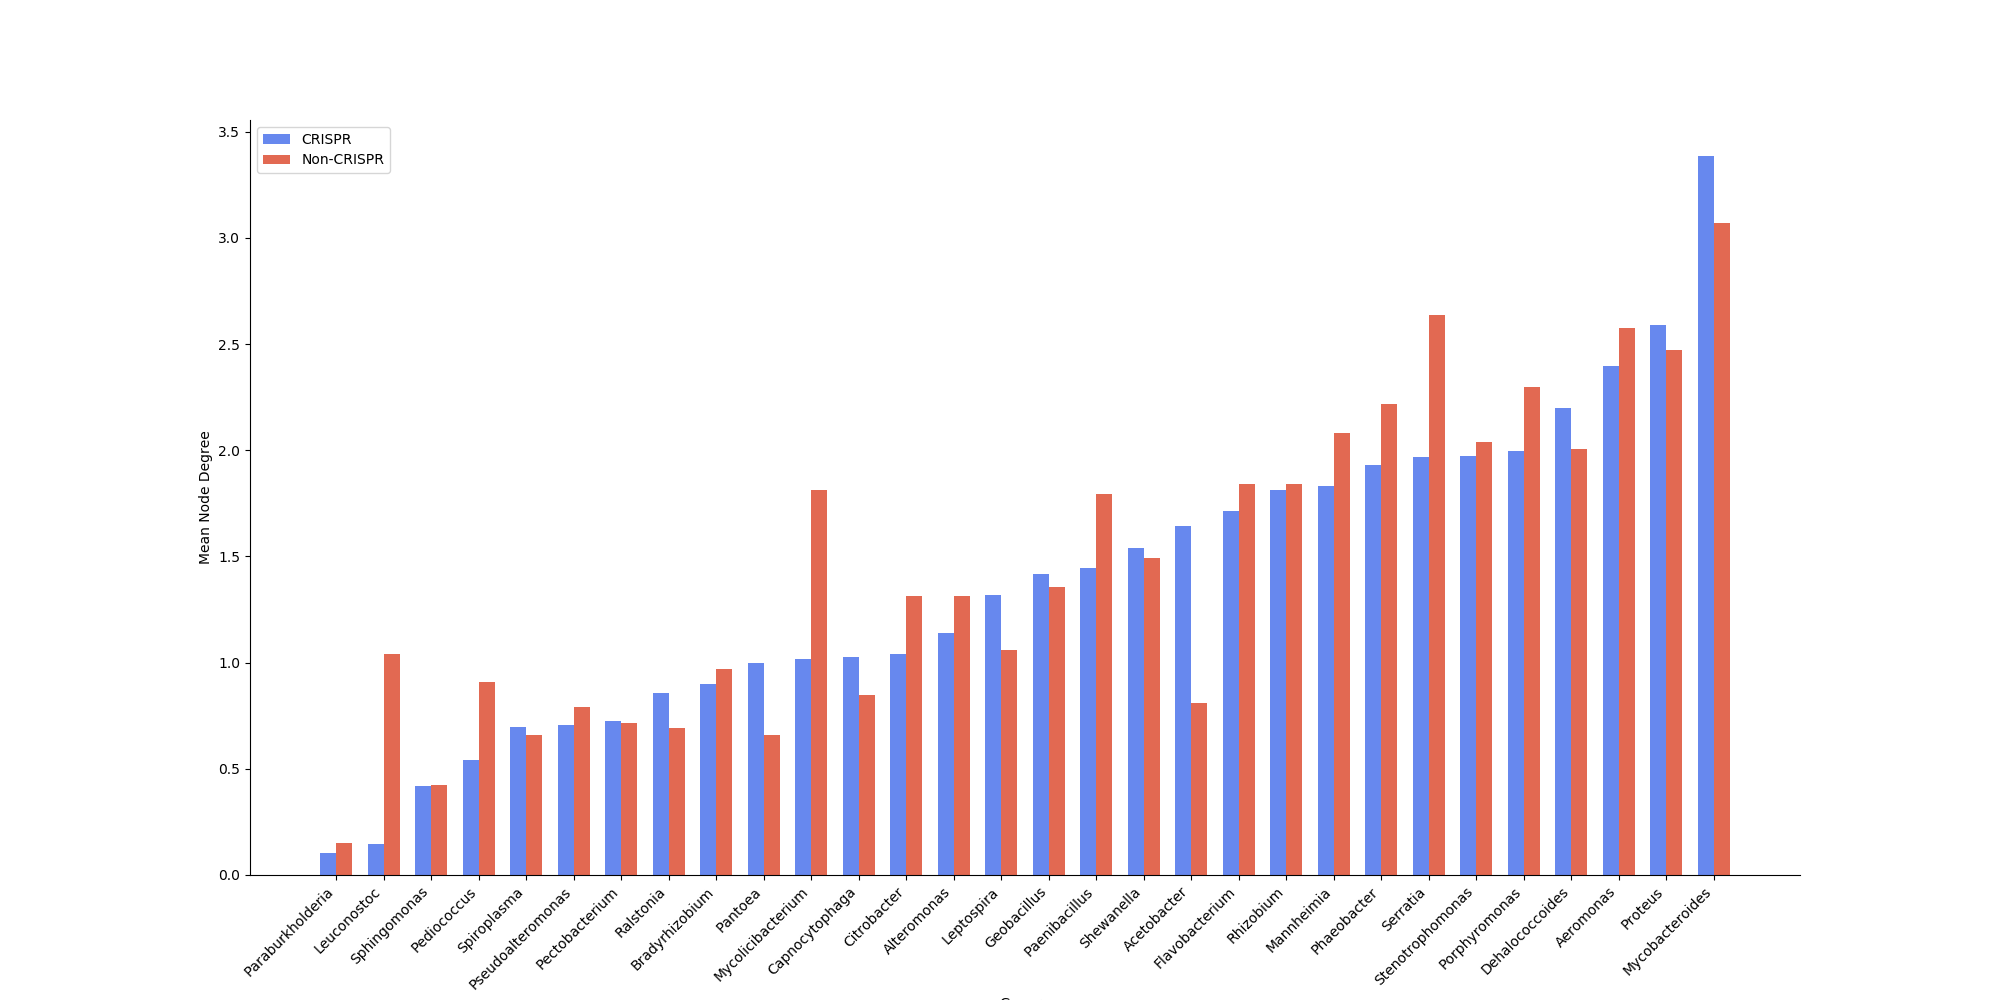
\includegraphics[width=\linewidth]{c_nc_deg_bar.png}}
    \caption{Mean node degree for either all \ac{crsp} or Non-\ac{crsp} nodes across all 1000 bootstrap replicates for each genus. There were 30 genera used.}
\end{figure}
\FloatBarrier
%indel bar
\FloatBarrier
\begin{figure}[htb!]
    \makebox[\textwidth][c]{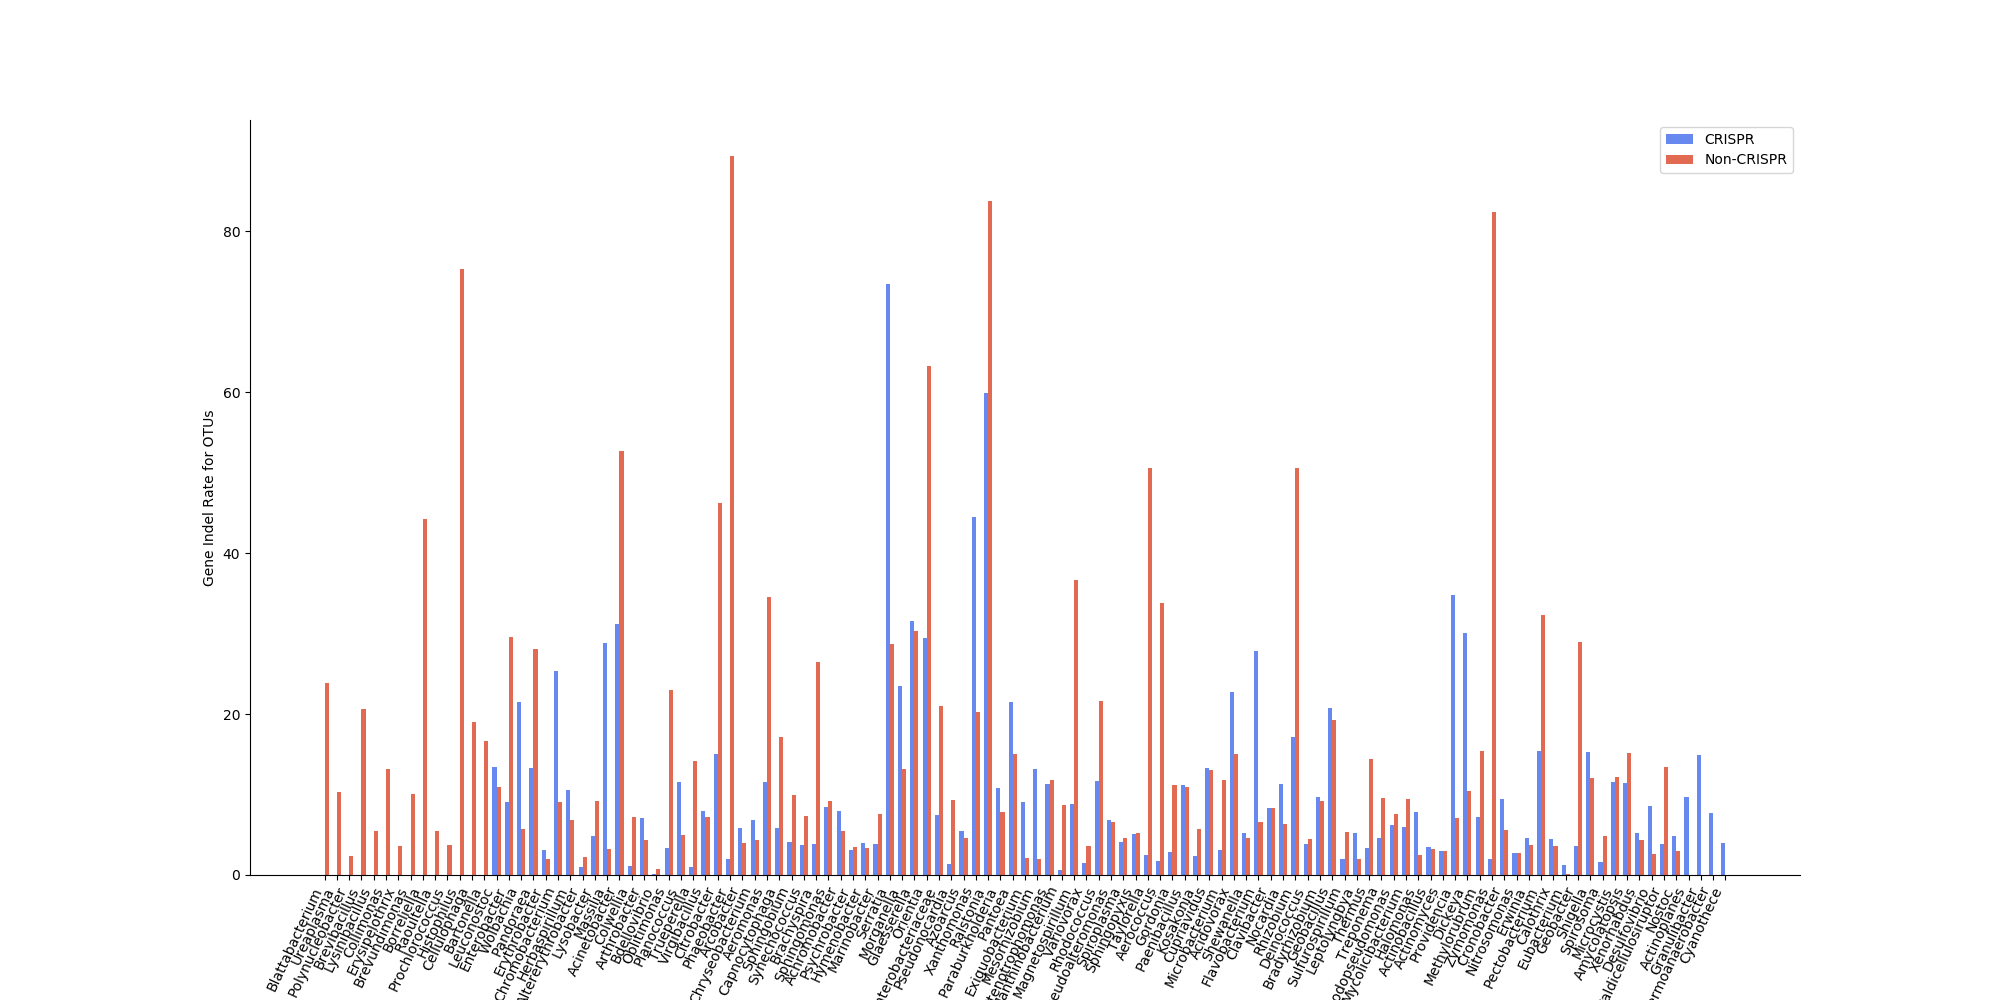
\includegraphics[width=\linewidth]{c_nc_indel_bar.png}}
    \caption{Markopholo estimate of gene indel rates for the partitions of \ac{crsp} and Non-\ac{crsp} \ac{otu}s for each genus. Rate is indel events per base pair substitution. There were 30 genera used.}
\end{figure}
\FloatBarrier
%indel scatter
\FloatBarrier
\begin{figure}[htb!]
    \makebox[\textwidth][c]{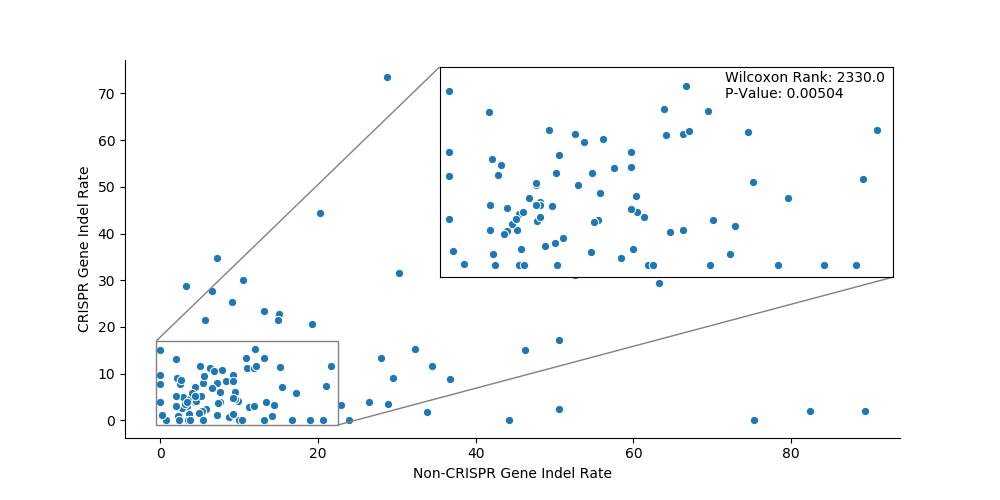
\includegraphics[width=\linewidth]{c_nc_rate_scatter.png}}
    \caption{Markopholo estimate of gene indel rates for the partitions of \ac{crsp} and Non-\ac{crsp} \ac{otu}s for each genus. Rate is indel events per base pair substitution. Each point represents a genus. There were 30 genera used.}
\end{figure}
\FloatBarrier
Wicoxon Signed Rank Test statistic and the asssociated p-value is show, implying a rejection of the null hypothesis that gene indel rates for \ac{crsp} and Non-\ac{crsp} \ac{otu}s are from
%Cfrac vs rate difference
\FloatBarrier
\begin{figure}[htb!]
    \makebox[\textwidth][c]{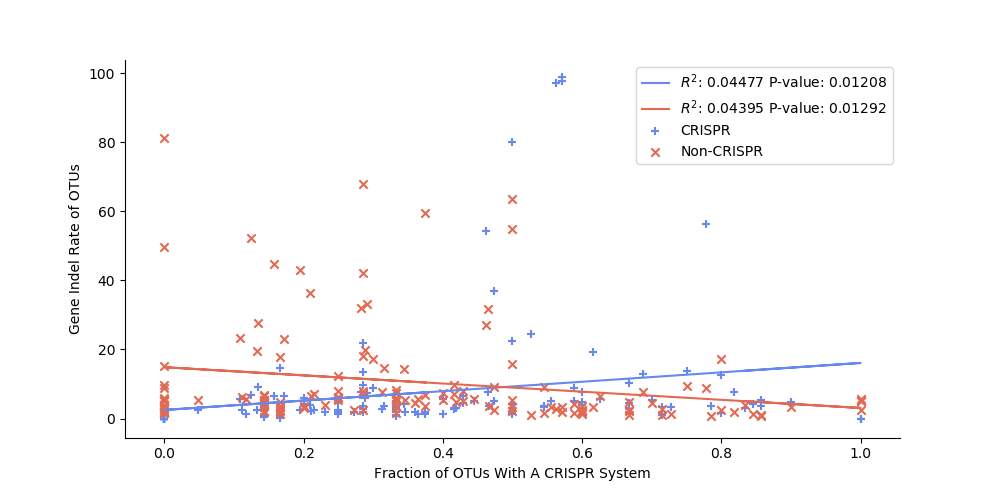
\includegraphics[width=\linewidth]{cfrac_cncRateDiff_scattter.png}}
    \caption{Markopholo estimate of gene indel rates for the partitions of \ac{crsp} and Non-\ac{crsp} \ac{otu}s for each genus against the fraction of all \ac{otu}s in that genus that are annotated as having a \ac{crsp} system. $R^2$ values are for linear regression lines fit to the \ac{crsp} and non-\ac{crsp} estimates. Rate is indel events per base pair substitution. Each point represents a genus. There were 30 genera used.}
\end{figure}
\FloatBarrier
%Cluster C NC
\FloatBarrier
\begin{figure}[htb!]
    \makebox[\textwidth][c]{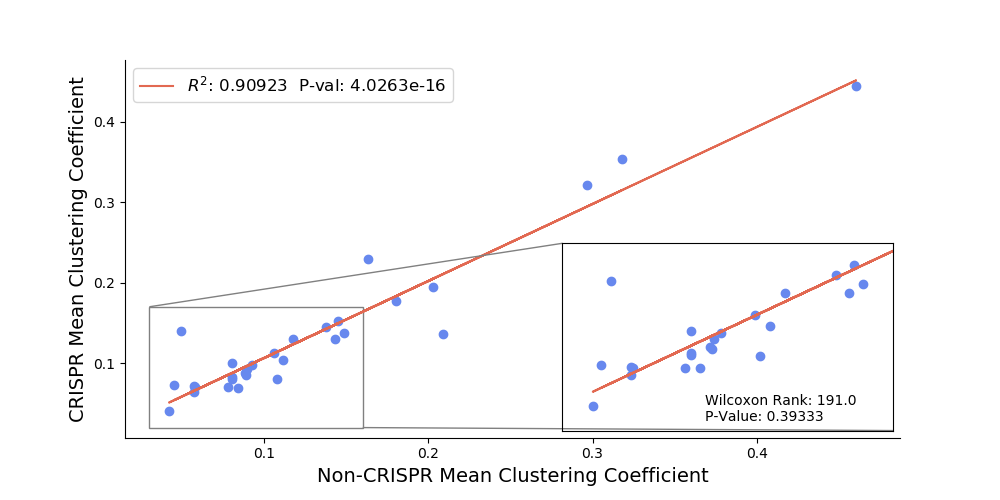
\includegraphics[width=\linewidth]{c_nc_clust_scatter.png}}
    \caption{Mean over 1000 bootstraps of the clutering coefficients of the \ac{crsp} \ac{otu}s for each genus against the non-\ac{crsp} means over the 1000 bootstraps. $R^2$ value is for the linear regression fit to the \ac{crsp} and non-\ac{crsp} estimates. There were 30 genera used.}
\end{figure}
\FloatBarrier
Wicoxon Signed Rank Test statistic and the asssociated p-value is show, implying a failure to reject of the null hypothesis that clustering coefficients for \ac{crsp} and Non-\ac{crsp} \ac{otu}s are from the same distribution
%modularity
\FloatBarrier
\begin{figure}[htb!]
    \makebox[\textwidth][c]{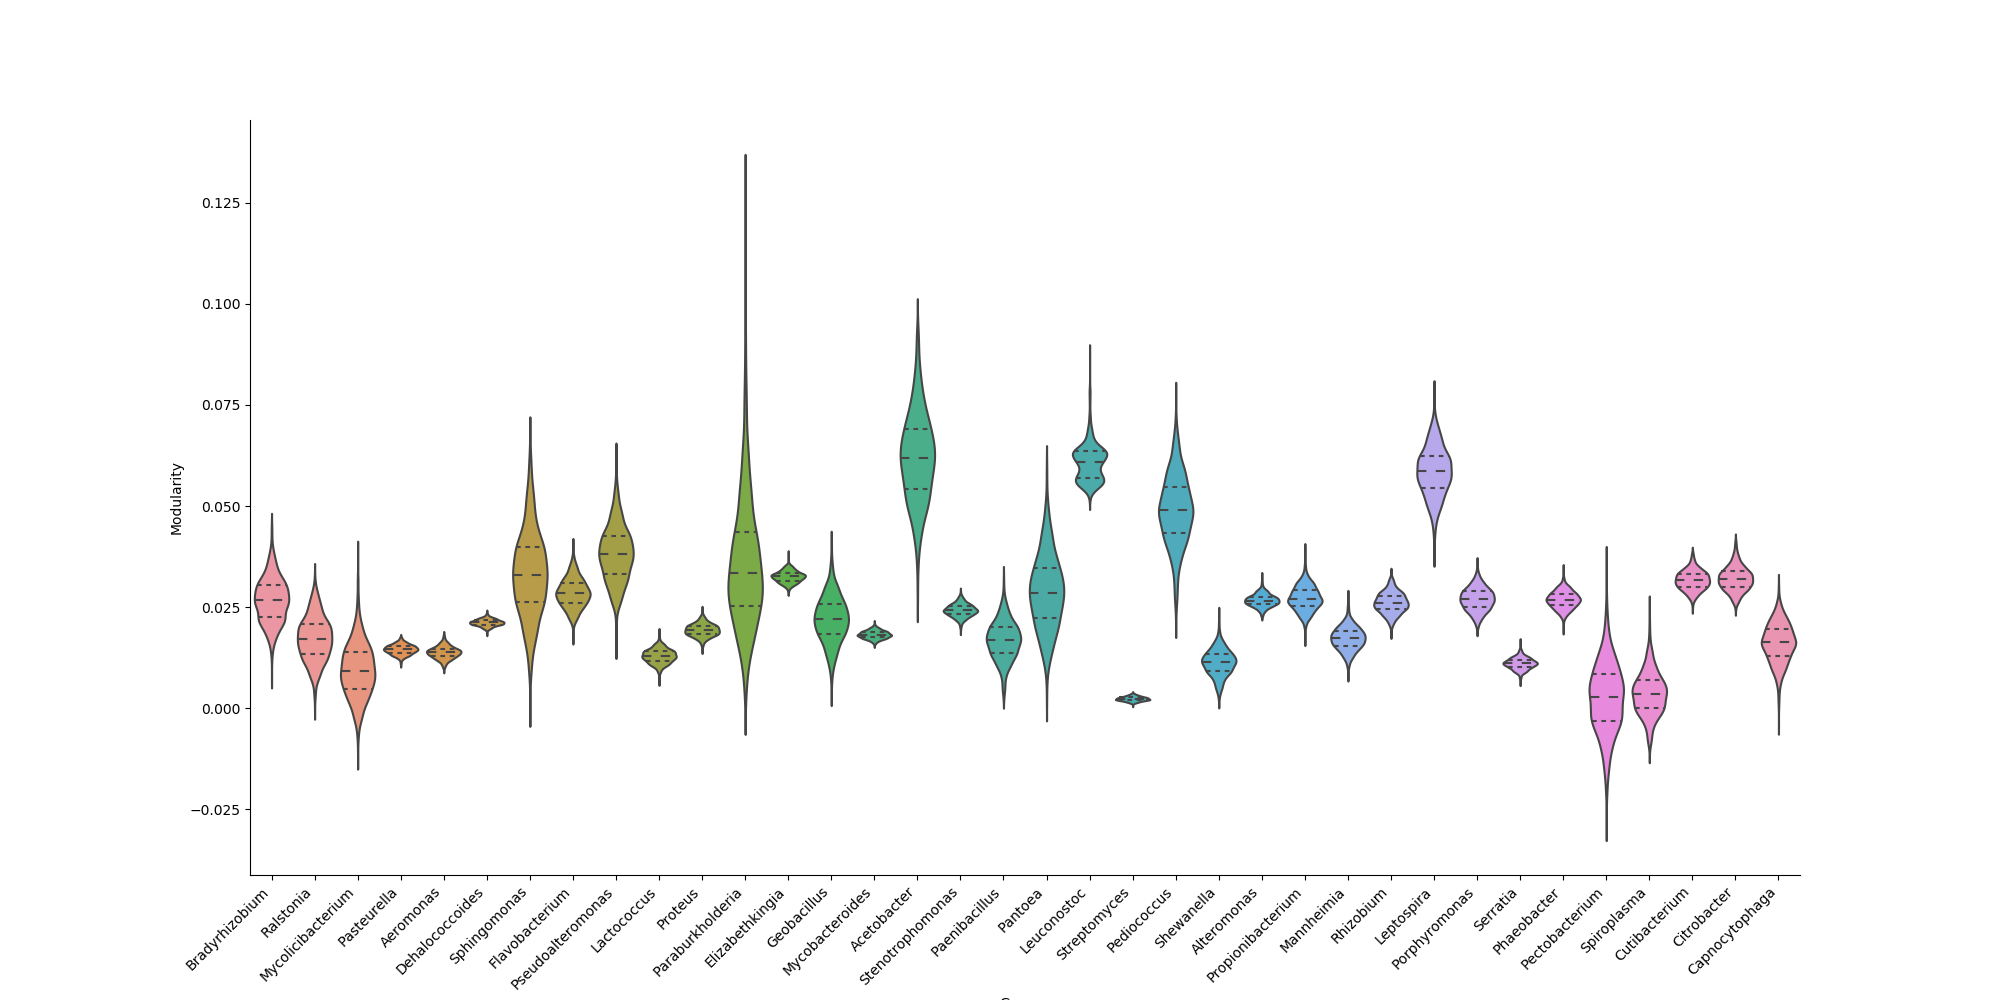
\includegraphics[width=\linewidth]{mod_violin.png}}
    \caption{Distribution of network modularity over 1000 bootstrap repliactes for each genus. Plot is of the kernel density estimated from the observed values, with witdh proportional to the number of data points. Lines inside each distribution represent quartiles.}
\end{figure}
\FloatBarrier
%Assortativity
\FloatBarrier
\begin{figure}[htb!]
    \makebox[\textwidth][c]{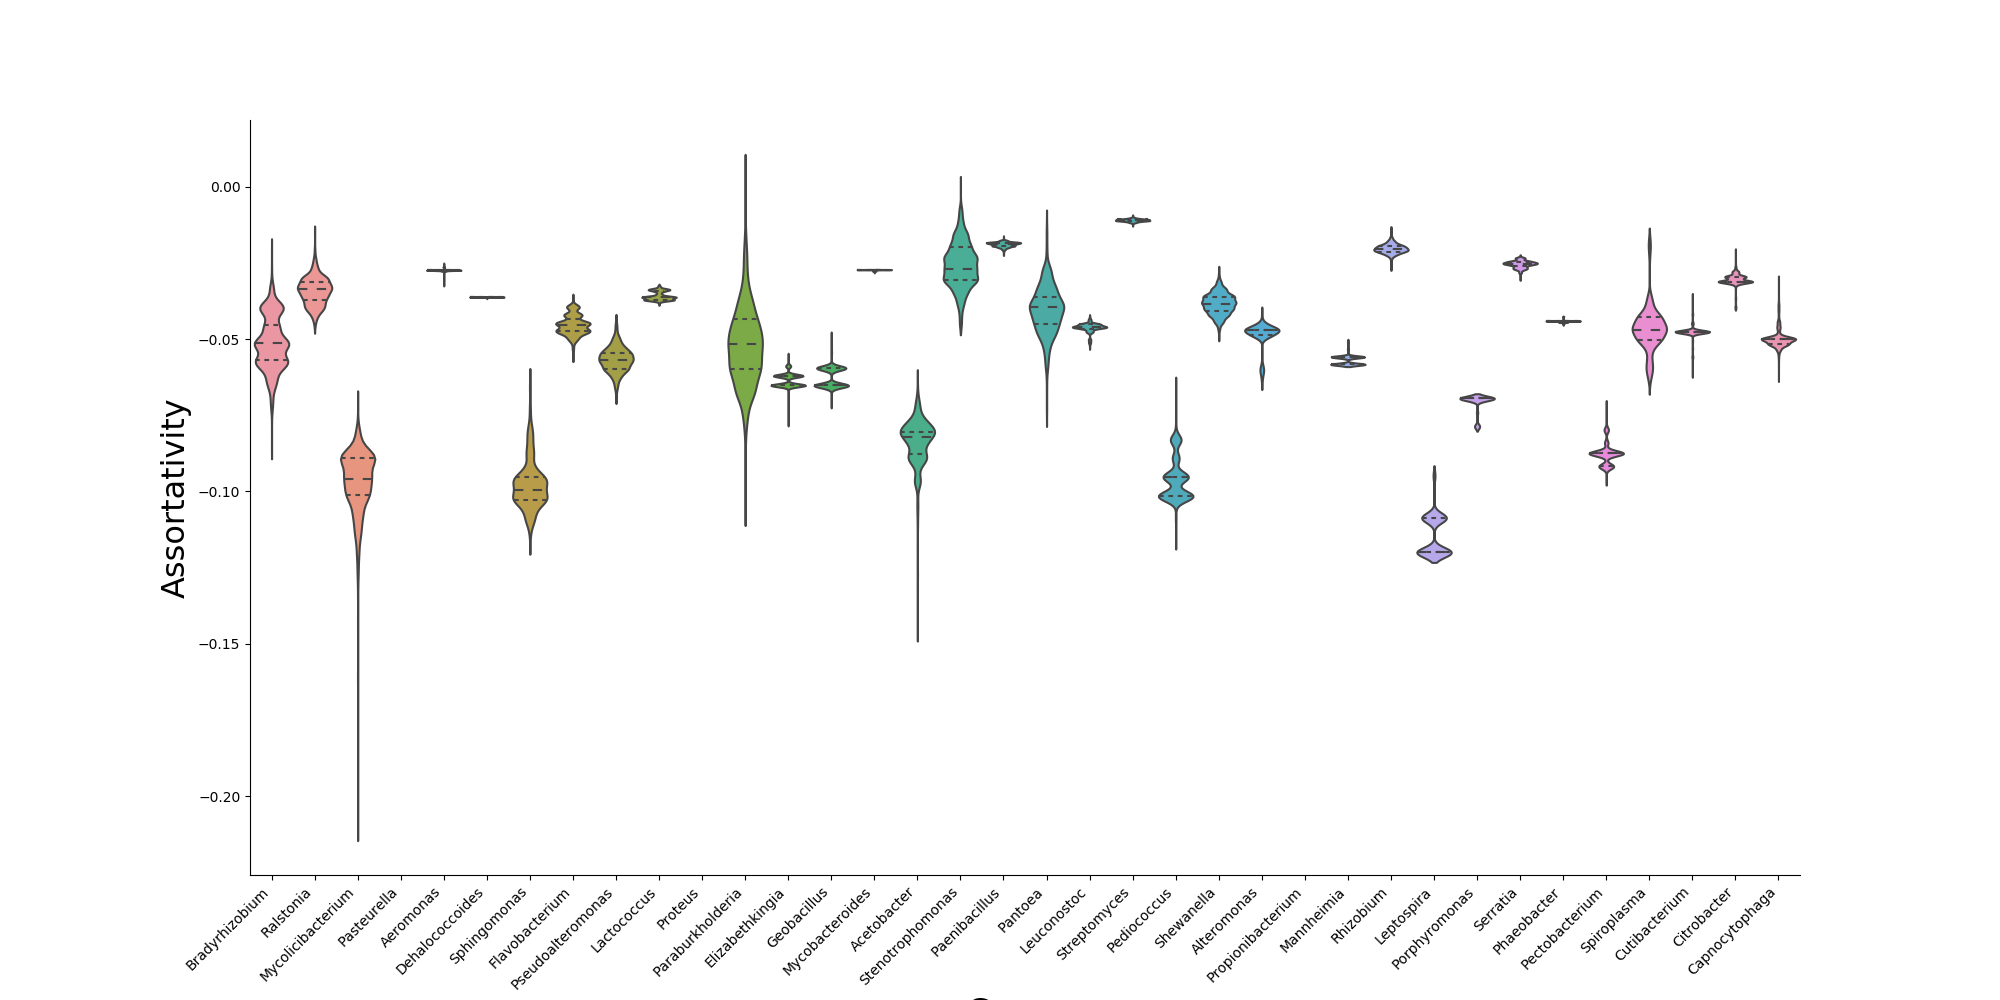
\includegraphics[width=\linewidth]{asst_violin.png}}
    \caption{Distribution of network assortativity by \ac{crsp} status (either \ac{crsp} or non-\ac{crsp}) over 1000 bootstrap repliactes for each genus. Plot is of the kernel density estimated from the observed values, with witdh proportional to the number of data points. Lines inside each distribution represent quartiles.}
\end{figure}
\FloatBarrier
%%pairplot
%\FloatBarrier
%\begin{figure}[htb!]
%    \makebox[\textwidth][c]{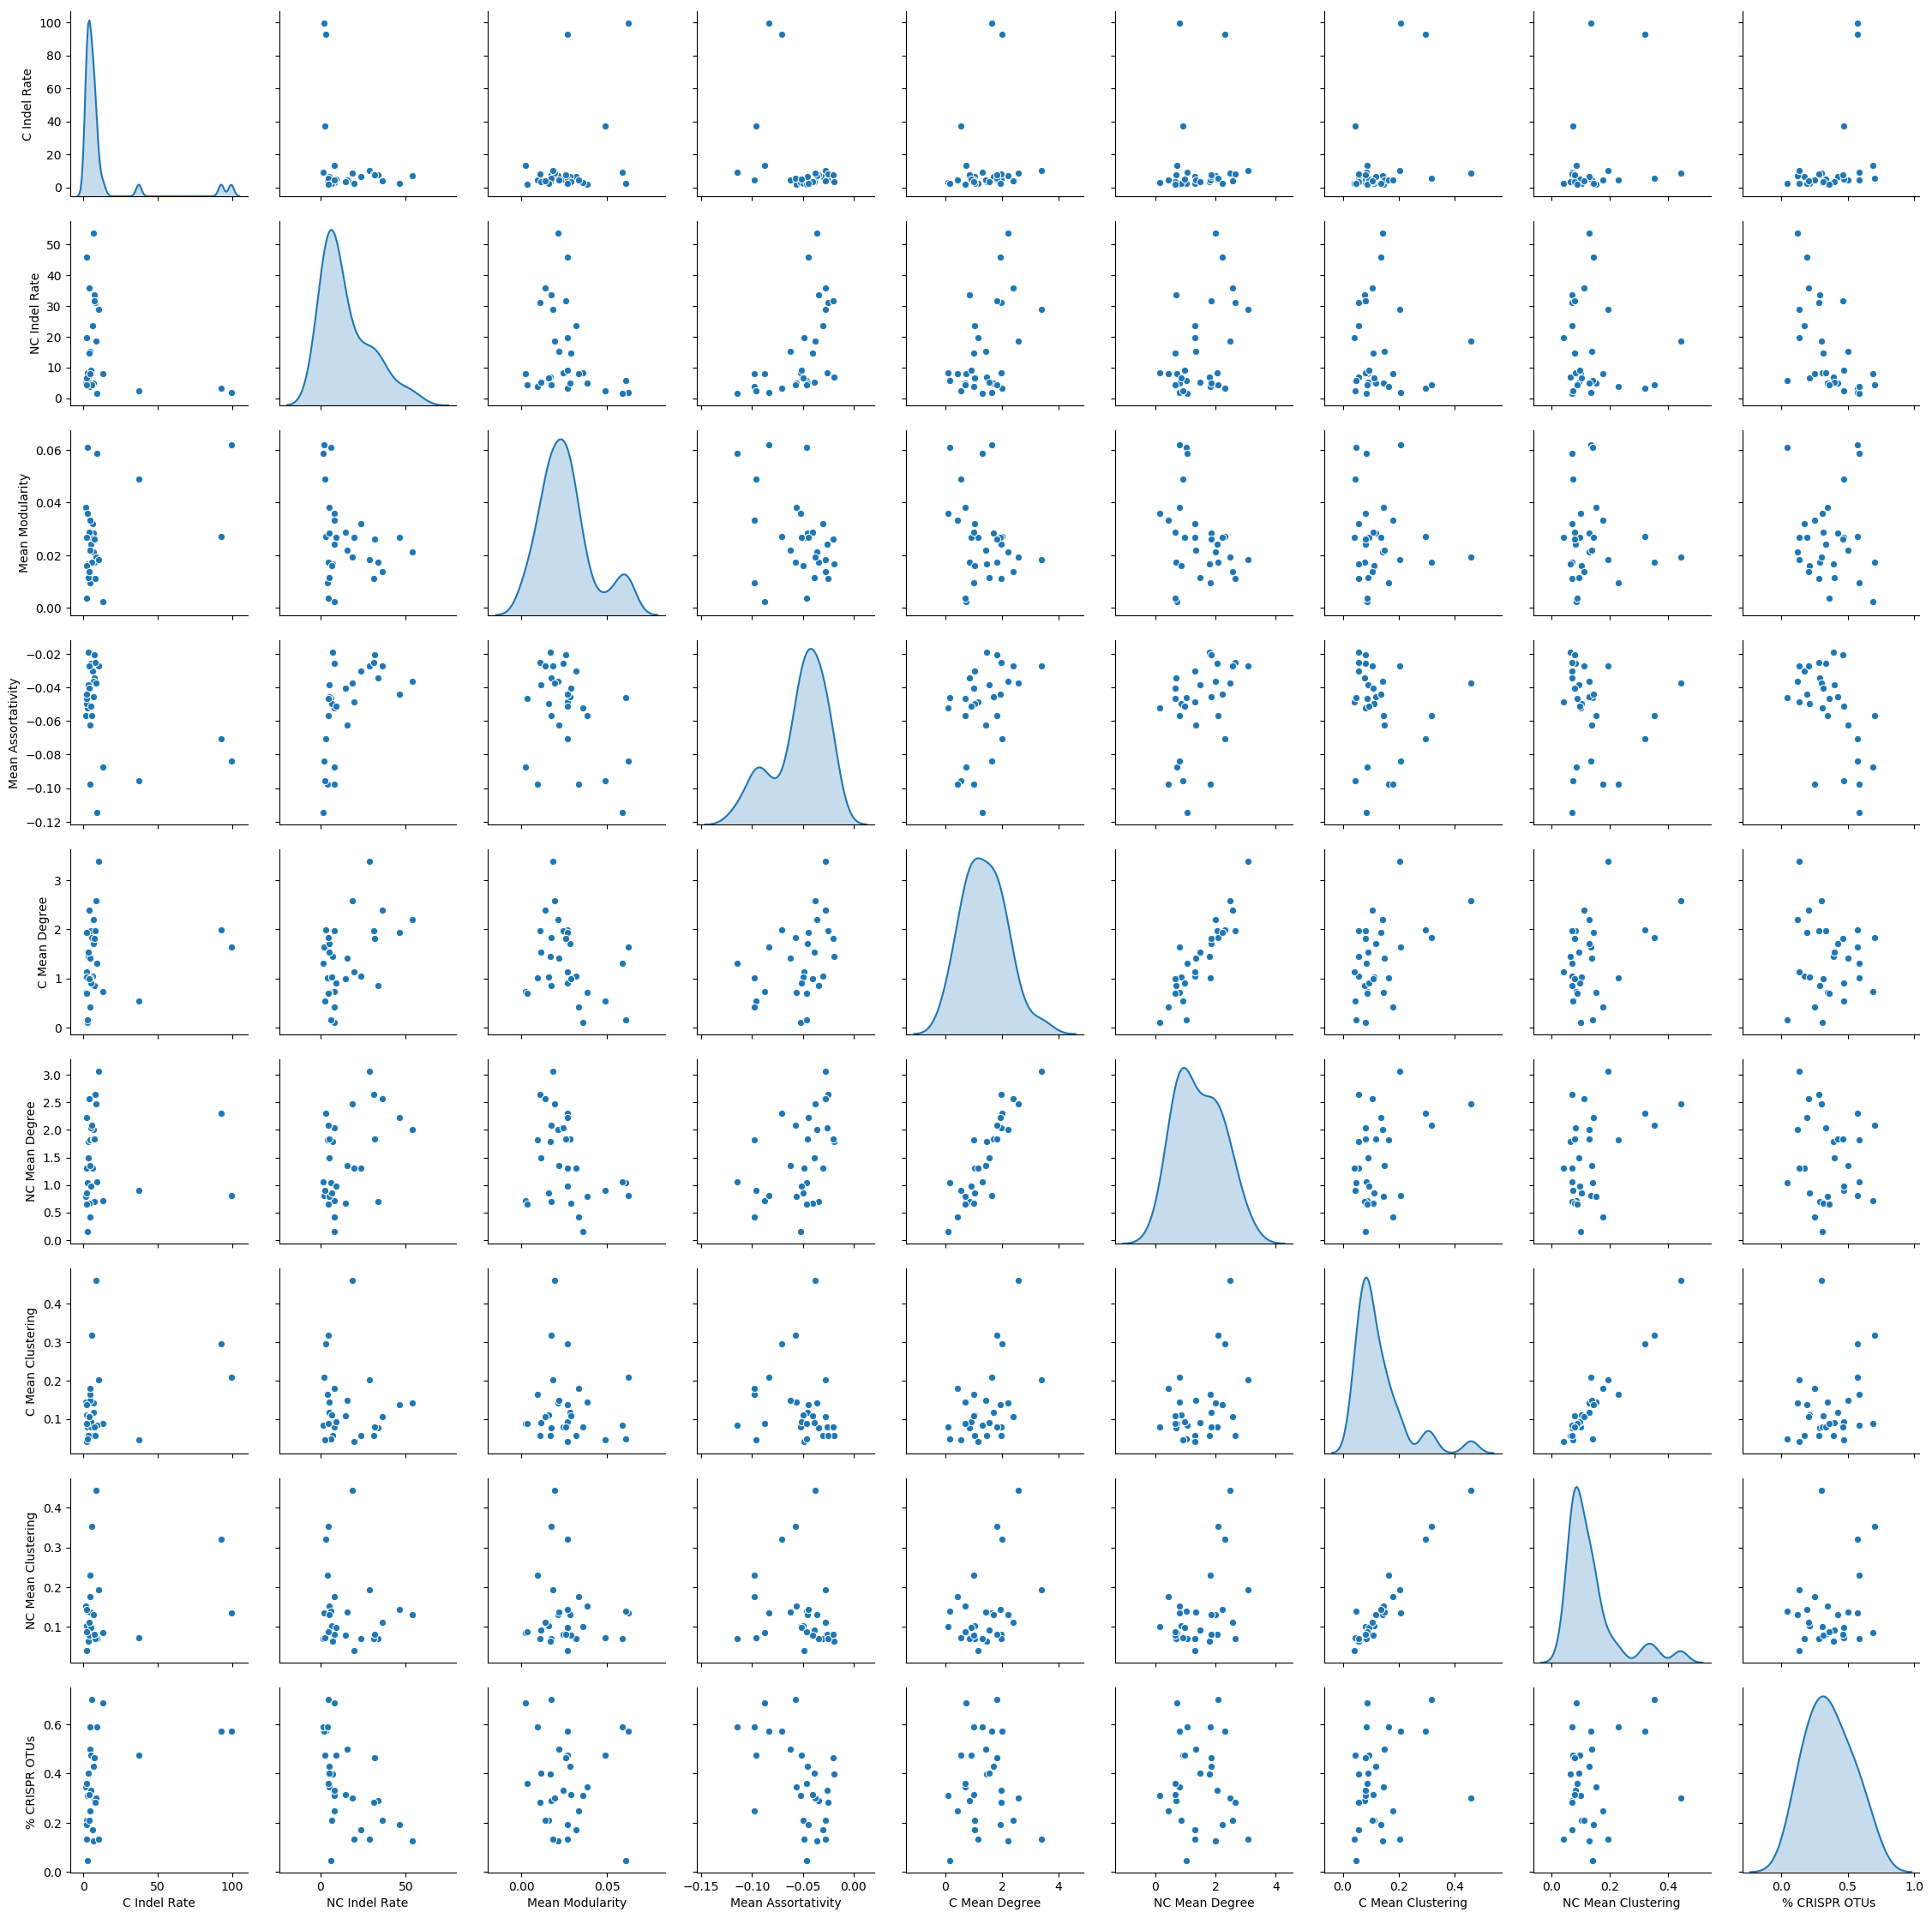
\includegraphics[width=\linewidth]{pairplot.png}}
%\end{figure}
%\FloatBarrier
